\documentclass[8pt,a4paper,compress]{beamer}

\usepackage{/home/siyer/lib/slides}

\title{Priority Queues}
\date{}

\begin{document}
\begin{frame}
\vfill
\titlepage
\end{frame}

\begin{frame}
\frametitle{Outline}
\tableofcontents
\end{frame}

\section{API}
\begin{frame}[fragile]
Many applications require that we process items having keys in order, but not necessarily in full sorted order and not necessarily all at once

\bigskip

An appropriate data structure in such applications is the priority queue (PQ for short), which supports two operations: insert and remove the minimum (or maximum)

\begin{center}
\begin{tabular}{cc}
method & description \\ \hline
\lstinline$MinPQ(int capacity)$ & constructs an empty PQ with the given initial capacity \\
\lstinline$MinPQ()$ & constructs an empty PQ \\
\lstinline$boolean isEmpty()$ & is the PQ empty? \\
\lstinline$int size()$ & number of keys in the PQ \\
\lstinline$void insert(Key v)$ & insert a key $v$ into the PQ \\
\lstinline$Key min()$ & return the smallest key in the PQ \\
\lstinline$Key delMin()$ & return and remove the smallest key in the PQ \\
\lstinline$Iterator<Item> iterator()$ & returns an iterator over the keys in the PQ in ascending order \\
$\dots$ & $\dots$
\end{tabular} 
\end{center}

\smallskip

\begin{center}
\begin{tabular}{cc}
method & description \\ \hline
\lstinline$MaxPQ(int capacity)$ & constructs an empty PQ with the given initial capacity \\
\lstinline$MaxPQ()$ & constructs an empty PQ \\
\lstinline$Key max()$ & return the largest key in the PQ \\
\lstinline$Key delMax()$ & return and remove the largest key in the PQ \\
\lstinline$Iterator<Item> iterator()$ & returns an iterator over the keys in the PQ in descending order \\
$\dots$ & $\dots$
\end{tabular} 
\end{center}
\end{frame}

\begin{frame}[fragile]
A \lstinline{MinPQ} client
\begin{lstlisting}[language=Java]
import edu.princeton.cs.algs4.*;

public class TopM {   
    public static void main(String[] args) {
        int M = Integer.parseInt(args[0]); 
        MinPQ<Transaction> pq = new MinPQ<Transaction>(M + 1); 
        while (StdIn.hasNextLine()) {
            String line = StdIn.readLine();
            Transaction transaction = new Transaction(line);
            pq.insert(transaction); 
            if (pq.size() > M) { 
                pq.delMin(); 
            }
        }
        Stack<Transaction> stack = new Stack<Transaction>();
        for (Transaction transaction : pq) { 
            stack.push(transaction); 
        }
        for (Transaction transaction : stack) {
            StdOut.println(transaction); 
        } 
    }
} 
\end{lstlisting} 

\begin{lstlisting}[language={}]
$ more tinyBatch.txt 
Turing      6/17/1990   644.08
vonNeumann  3/26/2002  4121.85
...
$ java TopM 5 < tinyBatch.txt 
Thompson    2/27/2000  4747.08
vonNeumann  2/12/1994  4732.35
vonNeumann  1/11/1999  4409.74
Hoare       8/18/1992  4381.21
vonNeumann  3/26/2002  4121.85
\end{lstlisting} 
\end{frame}

\section{Elementary Implementations}
\begin{frame}[fragile]
Elementary implementations of priority queues involve arrays or linked lists, ordered or unordered, which have the property that either the insert or remove the minimum (or maximum) operation takes linear time in the worst case

\bigskip

The heap data structure that we consider next enables implementations where both operations are guaranteed to be fast

\bigskip

Worst-case running time for priority-queue implementations
\begin{center}
\begin{tabular}{ccc}
data structure & insert & remove minimum (or maximum) \\ \hline \\
ordered array & $N$ & 1 \\
unordered array & 1 & $N$ \\
ordered linked list & $N$ & 1 \\
unordered linked list & 1 & $N$ \\
heap & $\log N$ & $\log N$ \\
impossible & 1 & 1
\end{tabular} 
\end{center}
\end{frame}

\section{Heap Definitions}
\begin{frame}[fragile]
A \emph{binary tree} is a tree data structure in which each node has at most two children

\bigskip

A \emph{maximum-oriented heap-ordered binary tree} is a binary tree in which each node is larger than or equal to the keys in that node's two children (if any)

\bigskip

The largest key in a maximum-oriented heap-ordered binary tree is found at the root

\bigskip

A \emph{binary heap} is a collection of keys arranged in a complete heap-ordered binary tree, represented in level order in an array (not using the first entry)

\begin{center}
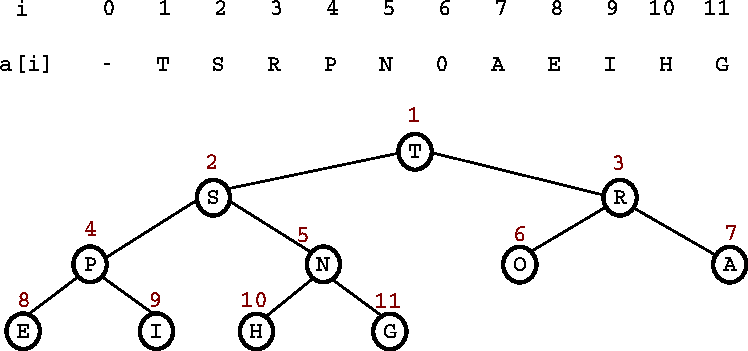
\includegraphics[scale=0.6]{{./figures/heap_representation}.pdf}

\smallskip

\tiny A binary heap
\end{center}

\bigskip

The height of a complete binary tree of size $N$ is $\floor{\log N}$
\end{frame}

\section{Algorithms on Heaps}
\begin{frame}[fragile]
Bottom-up reheapify (swim): if the maximum-oriented heap order is violated because a node's key is larger than its parent's key, we can fix the violation by exchanging the node with its parent, until we reach a node with a larger key, or the root

\bigskip

\begin{minipage}{150pt}
\begin{lstlisting}[language=Java]
private void swim(int k) {
    while (k > 1 && less(k / 2, k)) { 
        exch(k, k / 2); 
        k = k / 2; 
    }
}
\end{lstlisting}
\end{minipage}%
\begin{minipage}{130pt}
\hfill 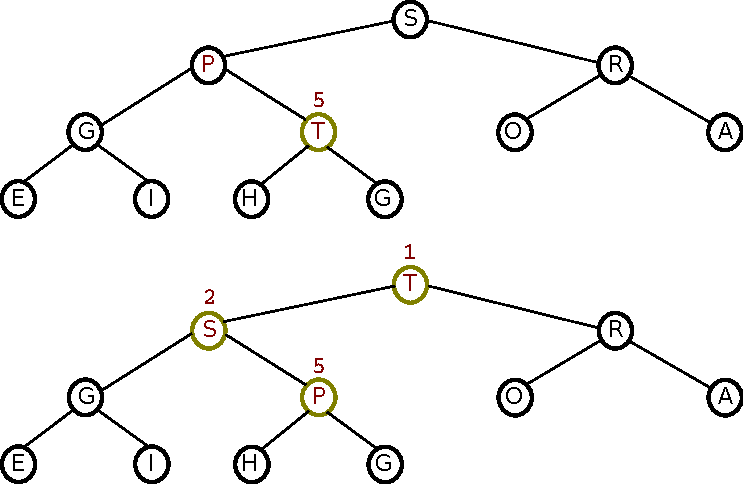
\includegraphics[scale=0.35]{./figures/heapify_swim.pdf}
\end{minipage}

\smallskip

\begin{center}
\tiny {Swim operation in a maximum-oriented heap-ordered binary tree}
\end{center}

\bigskip

Insert: add the new key at the end of the array, increment the size of the heap, and then swim up through the heap with that key to restore the heap condition
\end{frame}

\begin{frame}[fragile]
Top-down reheapify (sink): if the maximum-oriented heap order is violated because a node's key is smaller than one or both of its childrens' keys, we can fix the violation by exchanging the node with the larger of its two children, until we reach a node with both children smaller or equal, or the bottom 

\bigskip

\begin{minipage}{150pt}
\begin{lstlisting}[language=Java]
private void sink(int k) {
    while (2 * k <= N) {
        int j = 2 * k;
        if (j < N && less(j, j + 1)) { 
            j++; 
        }
        if (!less(k, j)) { break; }
        exch(k, j);
        k = j;
    }
}
\end{lstlisting}
\end{minipage}%
\begin{minipage}{130pt}
\hfill 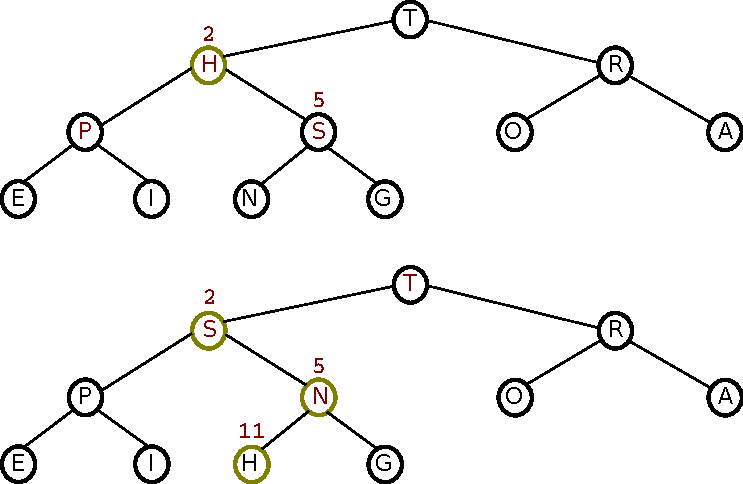
\includegraphics[scale=0.35]{./figures/heapify_sink.pdf}
\end{minipage}

\smallskip

\begin{center}
\tiny Sink operation in a maximum-oriented heap-ordered binary tree
\end{center}

\bigskip

Remove the maximum: take the largest key off the top, put the item from the end of the heap at the top, decrement the size of the heap, and then sink down through the heap with that key to restore the heap condition
\end{frame}

\begin{frame}[fragile]
\begin{lstlisting}[language=Java]
package edu.princeton.cs.algs4;

import java.util.Comparator;
import java.util.Iterator;
import java.util.NoSuchElementException;

public class MaxPQ<Key> implements Iterable<Key> {
    private Key[] pq;
    private int N;
    private Comparator<Key> comparator; 
    
    public MaxPQ(int capacity) {
        pq = (Key[]) new Object[capacity + 1];
        N = 0;
    }

    public MaxPQ() { this(1); }
    
    public boolean isEmpty() { return N == 0; }

    public int size() { return N; }

    public void insert(Key x) {
        if (N >= pq.length - 1) { resize(2 * pq.length); }
        pq[++N] = x;
        swim(N);
    }

    public Key max() {
        if (isEmpty()) { throw new NoSuchElementException("..."); }
        return pq[1];
    }
\end{lstlisting}
\end{frame}

\begin{frame}[fragile]
\begin{lstlisting}[language=Java]    
    public Key delMax() {
        if (isEmpty()) { throw new NoSuchElementException("..."); }
        Key max = pq[1];
        exch(1, N--);
        sink(1);
        pq[N + 1] = null; 
        if ((N > 0) && (N == (pq.length - 1) / 4)) { resize(pq.length / 2); }
        return max;
    }
    
    public Iterator<Key> iterator() { return new HeapIterator(); }
    
    private class HeapIterator implements Iterator<Key> {
        private MaxPQ<Key> copy;

        public HeapIterator() {
            if (comparator == null) { copy = new MaxPQ<Key>(size()); }
            else { copy = new MaxPQ<Key>(size(), comparator); }
            for (int i = 1; i <= N; i++) { copy.insert(pq[i]); }
        }

        public boolean hasNext() { return !copy.isEmpty(); }

        public Key next() {
            if (!hasNext()) { throw new NoSuchElementException(); }
            return copy.delMax();
        }
        ...
    }
    ...
}
\end{lstlisting}
\end{frame}

\begin{frame}[fragile]
In an $N$-key priority queue, the heap algorithms require no more than $1 + \lg N$ comparisons for insert and no more than $2 \lg N$ comparisons for remove the minimum (or maximum)

\bigskip

It is not difficult to modify our code to build heaps based on an array representation of complete heap-ordered ternary trees, and not much more difficult to use $d$-ary heaps for any given $d$

\bigskip

The priority queue contains objects that are created by clients but assumes that client code does not change the keys (which might invalidate the heap-order invariant)

\bigskip

In many applications, it makes sense to allow clients to refer to items that are already on the priority queue 
\begin{center}
\begin{tabular}{cc}
method & description \\ \hline
\lstinline$IndexMinPQ(int maxN)$ & \makecell{creates an empty indexed PQ with \\ indices $\in [0, maxN - 1]$} \\
\lstinline$void insert(int k, Item item)$ & insert $item$; associate it with $k$ \\
\lstinline$void change(int k, Item item)$ & change item associated with $k$ to $item$ \\
\lstinline$boolean contains(int k)$ & is $k$ associated with some item? \\
\lstinline$void delete(int k)$ & remove $k$ and its associated item \\
\lstinline$int minIndex()$ & return a minimal item's index \\
$\dots$ & $\dots$
\end{tabular} 
\end{center}
\end{frame}

\begin{frame}[fragile]
An \lstinline{IndexMinPQ} client
\begin{lstlisting}[language=Java]
import edu.princeton.cs.algs4.*;

public class Multiway { 
    private static void merge(In[] ins) { 
        int N = ins.length; 
        IndexMinPQ<String> pq = new IndexMinPQ<String>(N); 
        for (int i = 0; i < N; i++) { 
            if (!ins[i].isEmpty()) { pq.insert(i, ins[i].readString()); }
        } 
        while (!pq.isEmpty()) {
            StdOut.print(pq.minKey() + " "); 
            int i = pq.delMin(); 
            if (!ins[i].isEmpty()) { pq.insert(i, ins[i].readString()); }
        }
        StdOut.println();
    } 

    public static void main(String[] args) { 
        int N = args.length; 
        In[] ins = new In[N]; 
        for (int i = 0; i < N; i++) { ins[i] = new In(args[i]); } 
        merge(ins); 
    } 
} 
\end{lstlisting}

\begin{lstlisting}[language={}]
$ more m1.txt 
A B C F G I I Z
$ more m2.txt 
B D H P Q Q
$ more m3.txt 
A B E F J N
$ java Multiway m1.txt m2.txt m3.txt 
A A B B B C D E F F G H I I J N P Q Q Z 
\end{lstlisting}
\end{frame}

\section{Heap Sort}
\begin{frame}[fragile]
Insert all the items to be sorted into a minimum-oriented priority queue, then repeatedly remove the minimum to remove them all in order

\bigskip

To sort in place, heapify \lstinline$a[]$ containing $N$ items to a maximum-oriented heap-ordered binary tree, and repeatedly exchange the maximum key with the key at index $N$ and reheapify the first $N - 1$ keys 

\begin{lstlisting}[language=Java]
package edu.princeton.cs.algs4;

import java.util.Comparator;

public class Heap {
    ...
    public static void sort(Comparable[] a) {
        int N = a.length;
        for (int k = N / 2; k >= 1; k--) { sink(a, k, N); }
        while (N > 1) { exch(a, 1, N--); sink(a, 1, N); }
    }
    
    private static void sink(Comparable[] pq, int k, int N) {
        while (2 * k <= N) {
            int j = 2 * k;
            if (j < N && less(pq, j, j + 1)) { j++; }
            if (!less(pq, k, j)) { break; }
            exch(pq, k, j);
            k = j;
        }
    }
    ...
}
\end{lstlisting}

\bigskip

Heap sort uses fewer than $2N \lg N + 2N$ comparisons and $N\lg N + N$ exchanges to sort $N$ items
\end{frame}
\end{document}
